%%
%% This is file `sample-acmsmall-conf.tex',
%% generated with the docstrip utility.
%%
%% The original source files were:
%%
%% samples.dtx  (with options: `all,proceedings,bibtex,acmsmall-conf')
%% 
%% IMPORTANT NOTICE:
%% 
%% For the copyright see the source file.
%% 
%% Any modified versions of this file must be renamed
%% with new filenames distinct from sample-acmsmall-conf.tex.
%% 
%% For distribution of the original source see the terms
%% for copying and modification in the file samples.dtx.
%% 
%% This generated file may be distributed as long as the
%% original source files, as listed above, are part of the
%% same distribution. (The sources need not necessarily be
%% in the same archive or directory.)
%%
%%
%% Commands for TeXCount
%TC:macro \cite [option:text,text]
%TC:macro \citep [option:text,text]
%TC:macro \citet [option:text,text]
%TC:envir table 0 1
%TC:envir table* 0 1
%TC:envir tabular [ignore] word
%TC:envir displaymath 0 word
%TC:envir math 0 word
%TC:envir comment 0 0
%%
%% The first command in your LaTeX source must be the \documentclass
%% command.
%%
%% For submission and review of your manuscript please change the
%% command to \documentclass[manuscript, screen, review]{acmart}.
%%
%% When submitting camera ready or to TAPS, please change the command
%% to \documentclass[sigconf]{acmart} or whichever template is required
%% for your publication.
%%
%%
\documentclass{article}
%%

\usepackage{graphicx}
\usepackage{booktabs}
\usepackage{caption}
\usepackage{threeparttable}
\captionsetup[table]{skip=5pt} % Ajusta el 'skip' a los puntos que desees
%%
%% end of the preamble, start of the body of the document source.
\begin{document}

%%
%% The "title" command has an optional parameter,
%% allowing the author to define a "short title" to be used in page headers.
% \title{Dashboard Visualization}
%%
%% The "author" command and its associated commands are used to define
%% the authors and their affiliations.
%% Of note is the shared affiliation of the first two authors, and the
%% "authornote" and "authornotemark" commands
%% used to denote shared contribution to the research.
\author{Arturo Olivares Martos\and Lisa Pawlowski\and Mohamed Abdelmagied\and Kaimao Sheng\and Irene-Angelica Chounta}
\date{}

%%
%% By default, the full list of authors will be used in the page
%% headers. Often, this list is too long, and will overlap
%% other information printed in the page headers. This command allows
%% the author to define a more concise list
%% of authors' names for this purpose.
%\renewcommand{\shortauthors}{Trovato et al.}

%%
%% The abstract is a short summary of the work to be presented in the
%% article.
%%
%% This command processes the author and affiliation and title
%% information and builds the first part of the formatted document.
% \maketitle
%% MUC OUTLINE

\begin{figure}
  \centering
  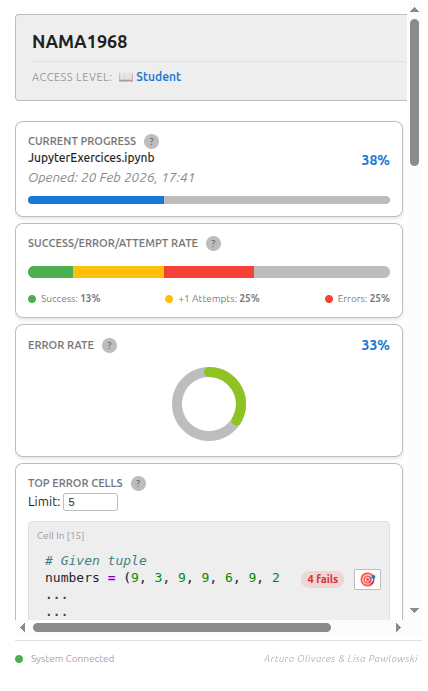
\includegraphics[width=1.0\textwidth]{general.png}
  \caption{General overview of the dashboard}
\end{figure}

\begin{figure}
  \centering
  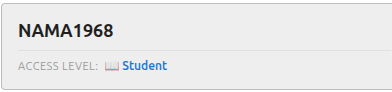
\includegraphics[width=1.0\textwidth]{user_info.png}
  \caption{User information panel}
\end{figure}

\begin{figure}
  \centering
  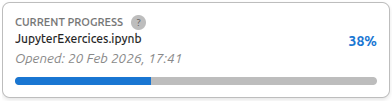
\includegraphics[width=1.0\textwidth]{current_progress.png}
  \caption{Current progress panel}
\end{figure}

\begin{figure}
  \centering
  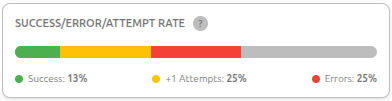
\includegraphics[width=1.0\textwidth]{success_error_attempt_rate.png}
  \caption{Success, error and attempt rate panel}
\end{figure}

\begin{figure}
  \centering
  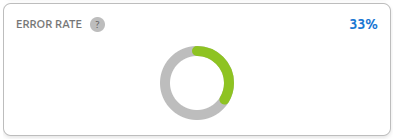
\includegraphics[width=1.0\textwidth]{error_rate.png}
  \caption{Error rate panel}
\end{figure}

\begin{figure}
  \centering
  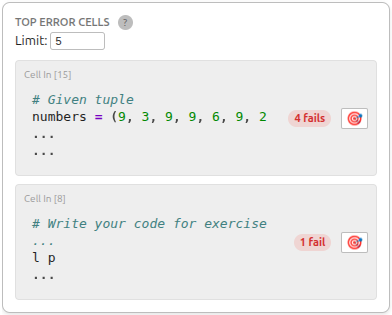
\includegraphics[width=1.0\textwidth]{top_error_cells.png}
  \caption{Top error cells panel}
\end{figure}

\begin{figure}
  \centering
  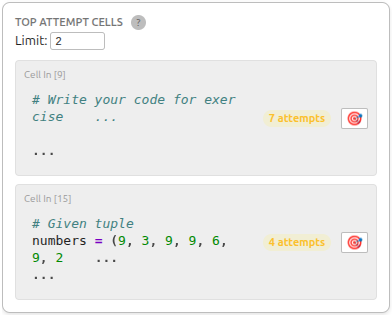
\includegraphics[width=1.0\textwidth]{top_attempt_cells.png}
  \caption{Top attempt cells panel}
\end{figure}

\begin{figure}
  \centering
  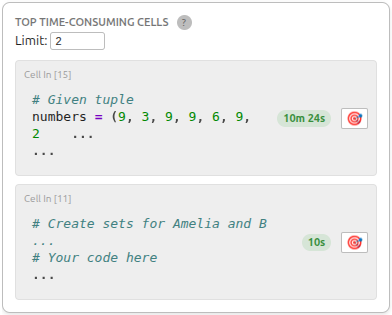
\includegraphics[width=1.0\textwidth]{top_time_consuming_cells.png}
  \caption{Top time consuming cells panel}
\end{figure}

\begin{figure}
  \centering
  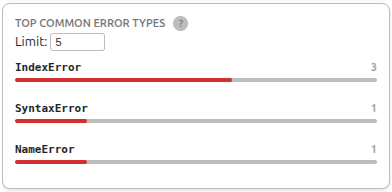
\includegraphics[width=1.0\textwidth]{top_common_error_types.png}
  \caption{Top common error types panel}
\end{figure}

\begin{figure}
  \centering
  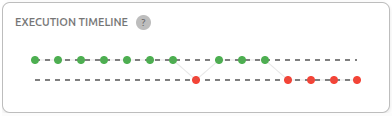
\includegraphics[width=1.0\textwidth]{./execution_timeline.png}
  \caption{Execution timeline panel}
\end{figure}




\end{document}
\endinput
%%
%% End of file `sample-acmsmall-conf.tex'.
